%%%%%%%%%%%%%%%%%%%%%%%%%%%%%%%%%%%%%%%%%%%%%%%%%%%%%%%%%%%%%%%%%%%%%%%%%%%%%%%%
% Diese Datei beinhaltet den eigentlichen Inhalt Ihrer Arbeit.
%
% Es bietet sich der Übersicht halber an, die einzelnen Abschnitte jeweils
% in eigene Dateien zu schreiben und mittels \input einzubinden.
% Eine mögliche Verzeichnisstruktur sähe entsprechend so aus:
%
% thesis/
% +- tex/
% |  +- introduction.tex
% |  +- motivation.tex
% |  +- experiments.tex
% |  |  ...
% |  +- conclusion.tex
% +- abstract.tex
% +- contents.tex
% +- thesis.tex
%%%%%%%%%%%%%%%%%%%%%%%%%%%%%%%%%%%%%%%%%%%%%%%%%%%%%%%%%%%%%%%%%%%%%%%%%%%%%%%%

% TODO
% [x] conclusions
% [ ] subsections should not be shorter than half a page
% [x] token span in parser section
% [x] hack vm erklären, bytecode (vielleicht mit stack bild)
% [x] abstract Neu
% [x] list of tested programs in appendix
% [x] user manual in readme
% [x] architektur schriftgröße erhöhen
% [x] bilder an korrekte stellen (keine bilder und co section mehr)
% [ ] write more about unit tests in compatability section
% [ ] rewrite sys.wait to return 1 as the second state or refer to the code
% [ ] explain dynamic dispatch (maybe glossary)
% [ ] intro to 6 and 7 is too similar
% [ ] explain hack archicture
% [ ] absolute jumps maybe not known
% [ ] benchmarks: speed for web is very browser/os dependent

% Feedback
% bytecode representation is hard to read
% too much explanation: error handling & macros

\section{Introduction}

Over the decades since its inception, the field of computer science has become increasingly complex and confusing.
This has caused students today to lose track of the picture at large and instead specialize on specific aspects of the field.
Shimon Schocken and Noam Nisam believe that this is an issue and that the best way to understand how computers actually work is to build one from scratch yourself.~\cite[Preface]{nisan2005}

In order to enable students to take this seemingly impossible approach, Schocken and Nisan developed the Nand to Tetris course in 2004, which gives students the opportunity to build an entire computer system themselves.~\cite{1408798}
The system the participants create over the course of twelve projects is powerful enough to allow for the implementation of complex applications and games.\ref{fig:hackenstein-offiziell}

To enable students to work on the included projects in a different order than intended, the authors included a hardware simulator to start with and two different emulators, which are capable of emulating the progress of the preceding projects.
Those emulators however are also a frequent point of criticism among course participants, as they increasingly no longer meet the demands of modern users.
Written in Java using the Swing Framework they are not only slow, but also do not adapt to today's higher display resolutions, making it difficult to actually see the contents of the running application.

It is therefore meaningful to rewrite those emulators in order to make the course more approachable and by extension increase the number of participants.

As part of this work, the two emulators were rewritten as a browser application using WebAssembly. This not only enables support for larger screens and significantly improved performance, but also allows the tools to be used without being installed on the the student's computer.

\section {Technologies}

\subsection{WebAssembly}

WebAssembly (abbreviated Wasm) is a binary instruction format for a stack-based virtual machine. It is designed as a portable compilation target for programming languages, enabling the usage of traditionally native languages, such as C/C++ or Rust for web development.~\cite{wasmweb}
Wasm however is not a replacement for JavaScript (JS) in its entirety. Rather it is intended to complement JS by being used to implement the computationally intensive parts of web applications, while all parts related to DOM manipulation and event handling continue to be written in JS.~\cite{wasmmdn}

\subsection{Rust}

Rust is a multi-paradigm programming language that tries to combine high-level ergonomics with low-level control. \cite[Introduction]{klabnik2019rust}
Besides the option to compile to native machine code, Rust is also capable of targeting Wasm as its platform, making it possible to use Rust for web development.~\cite{rustwasm}
Just like C and C++, Rust does not use runtime garbage collection by default, but unlike those langauges, Rust also does not require the programmer to explicitly free memory themselves.
Instead, it relies on its compiler to automatically insert all the necessary cleanup code. This is made possible by the ownership system, which tracks the lifetime of every reference in the program and ensures that nothing can be used after being freed.
In order to do this, the compiler has to enforce a set of rules, which will cause a compilation error if broken.~\cite[Chapter~4]{klabnik2019rust}
This unique approach allows achieving the same performance as C/C++, but without sacrificing memory safety.
However, it also has its drawbacks: When more rules are imposed on the programmer, writing and especially refactoring code tends to become more tedious, since a simple change from an owned object to a reference in Rust often requires inserting explicit lifetimes into large portions of the code base.

\subsection{The advantages of Rust and WebAssembly over JavaScript}

WebAssembly offers significant performance improvements over JavaScript, often reaching execution times within 10\% of native code. Even the optimized subset of JavaScript known as asm.js is, on average, 33.7\% slower than Wasm~\cite[Chapter~7.3]{wasmspeed}. The advantages do not stop with performance however, if used as a compilation target, it offers the ability to use Rust's powerful and versatile type system on the web.
This type system, inspired by ML and Haskell~\cite{rustinfluences}, provides programmers with a variety of ways to specify and limit the capabilities of certain types in their applications.
It enables the detection and prevention of entire classes of errors at compile time, dramatically reducing the amount of end-to-end testing required.
Some features in Rust's type system are especially valuable for writing emulators, namely Enums, Pattern Matching and Traits, whose influences on the design of the final application will be explained in further detail in \cref{implementation}.

\begin{itemize}
  \item Performance
  \item Stability und reliability through the rich typesystem and ownership model
  \item useful language features: Enums, Pattern Matching and Traits
  \item https://dl.acm.org/doi/abs/10.1145/3062341.3062363
  \item type system: inspired by ML and Haskell (https://doc.rust-lang.org/reference/influences.html)
\end{itemize}

\subsection{The advantages of Rust over other WebAssembly languages}

\begin{itemize}
  \item Performance and Bundle size (no GC, small runtime)
  \item stable ecosystem: wasm-bindgen, web-sys, console\_error\_panic\_hook
  \item stable language (multiple major releases, backwards compatibility)
  \item safer than C/C++ https://msrc-blog.microsoft.com/2019/07/16/a-proactive-approach-to-more-secure-code/
  \item good tooling: Cargo, Great error messages, editor support
\end{itemize}

\subsection{ReactJS}

\begin{itemize}
  \item Industry standard for reactive frontend development
  \item very stable and mature with tons of resources
\end{itemize}

\subsection{The advantages of ReactJS over pure JavaScript}

\begin{itemize}
  \item Component architecture simplifies code re-use
  \item simple, declarative and efficient updates for Components
  \item UI = f(state) instead of imperative spagetti code
\end{itemize}

\section{Related work}

\subsection{Nand to Tetris}
\begin{itemize}
  \item VM Bytecode design und high level Funktionalität
  \item CPU Assembly design und high level Funktionalität
  \item TST design und high level Funktionalität
  \item Viele Tests für Emulatoren aus N2T Projekten
\end{itemize}

\subsection{Dependencies}
\begin{itemize}
\item lazy\_static (hack um rust weniger nervig zu machen)
\item regex
\item wasm-bindgen (rust code für JS zugänglich machen)
\item web-sys (js stdlib in Rust nutzen)
\item console\_error\_panic\_hook (rust panics zu JS exeptions)
\item sdl2 (native UI (eigentlich nur zum Testen))
\item clap (CLI parsing)
\item wasm-pack (rust -> wasm Kompilierung einfacher machen)
\item react und npm (UI)
\end{itemize}

\subsection{Existing Nand to Tetris Emulator implementations}
\begin{itemize}
  \item https://github.com/itoshkov/nand2tetris-emu
  \item https://github.com/mossprescott/pynand
\end{itemize}

\subsection{Emulators in WebAssembly}
\begin{itemize}
  \item https://ieeexplore.ieee.org/abstract/document/9824078
  \item https://wasm4.org/
\end{itemize}

\section{Nand to Tetris und die Hack Architektur}
\subsection{Die Abschnitte des Nand to Tetris Kurses}
\begin{itemize}
  \item Chips und Logic Gates (nicht Teil der Arbeit)
  \item CPU und Assembly
  \item Virtuelle Machine
  \item High level Sprache und Betriebssystem (nicht Teil der Arbeit)
\end{itemize}

\subsection{Ein Überblick über VM Architektur im Allgemeinen}
\subsubsection{Beispiel: Zahlen in Schleife addieren in simpler VM}
\begin{lstlisting}[language=C, caption={Berechne 1 + 2 + 3 in C}, captionpos=b]
  int i = 1;
  int sum = 0;
  while (i <= 3) {
    sum += i;
    i++;
  }
\end{lstlisting}
\begin{lstlisting}[caption={Berechne 1 + 2 + 3 in einer Stack-basierten VM}, captionpos=b]
  // i = 1
  push 1
  pop i

  // sum = 0
  push 0
  pop sum

  label LOOP_START
  push i
  push 3
  // i <= 3 pusht entweder true oder false auf den stack
  less-than-or-equal
  // wenn der vorherige check false war, springen wir aus der Schleife
  goto-if-false LOOP_END

  // wenn i immer noch <= 3, addieren wir zuerst i und sum
  // und schreiben das Ergebnis der Addition wieder in die Summe
  push i
  push sum
  add
  pop sum

  push i
  push 1
  add
  pop i  // i = i + 1

  // Springe zum Anfang der Schleife
  goto LOOP_START

  label LOOP_END
\end{lstlisting}

\subsection{Hack Bytecode}
\subsubsection{Das obige Beispiel in der Hack Architektur}
\begin{lstlisting}[caption={Berechne 1 + 2 + 3 in der Hack VM}, captionpos=b]
  // i = 1
  push constant 1
  pop local 0

  // sum = 0
  push constant 0
  pop local 1

  label LOOP_START

  // die Hack Architektur besitzt keine <= Instruktion,
  // insofern benutzen wir i < 4 anstatt i <= 3
  push local 0
  push constant 4
  lt

  // falls i >= 4 ist springen wir aus der Schleife
  not
  if-goto LOOP_END

  // sum = sum + i
  push local 1
  push local 0
  add
  pop local 1

  // i = i + 1
  push local 0
  push constant 1
  add
  pop local 0

  // Springe zum Anfang der Schleife
  goto LOOP_START
  label LOOP_END
\end{lstlisting}

\section{Implementation} \label{implementation}

\subsection{General approach}
\subsubsection{Test driven development of the VM without an UI}
\begin{itemize}
  \item first implement bytecode parser, because it can be used in VM Tests
  \item basic VM features (everything except for function, call, return)
  \item testing with unit tests (Translations of VME.tst tests)
  \item rest of the VM instructions
  \item stdlib only as vm bytecode
\end{itemize}

\subsection{Architectural overview}
The general architecture of the application is outlined in \cref{fig:arch}.
There are three possible entry points for the application, which are listed in the interfaces section of the figure.

\subsection{VM development in Rust}
\subsection{Parser development in Rust}
\subsection{The test-script workflow}
\subsection{The native standard library protocol}
\subsection{Using conditional compilation in Rust}

\section{Evaluation} \label{evaluation}
When evaluating the success of a project, it is paramount to keep in mind the original goal of the project.
In this case, the primary goal was to provide an alternative VM emulator implementation to the participants of the Nand to Tetris course to make Project 9 and 12 more convenient.
Not only was this goal achieved, but in addition, the CPU emulator was also rewritten and both emulators have been integrated into a test-script-driven workflow, making them useful to course instructors.
Then again, projects do not exist in a vaccum, so the following sections contain a comprehensive comparison with the official emulator.

\subsection{Comparison with the official Emulator based on compatability} \label{compatibility}
It is impossible to test every existing program for the Hack VM, both due to the sheer volume of existing applications and the fact that many of these applications are not available to the public.
However, this is also not necessary, since the expected behavior of the emulators is clearly described in the book accompanying the course.
By following the specification and testing the new implementation with a reasonable number of representative programs, one can determine the degree of compatibility.
Those programs are listed in the appendix~\ref{table:tested}.
The number of possible instructions in the VM is also manageable, so a sufficiently complex program will use every single available instruction, which further supports this claim.
By and large, the new emulator behaves exactly like the old one.
This even applies to behaviors that could be considered bugs, such as the way the keyboard handler in the Java implementation interprets each letter as a capital letter, thus limiting the entire input system to uppercase letters.
This is not a technical limitation of either the VM or the Java input event, but simply a consequence of the implementation of the keyboard handler, and could easily be changed to allow lowercase letters as well.
But that would affect a number of existing applications, since they only check for uppercase letters in their game code, which means that those applications could no longer be used without problems.
For this reason, the new emulator also only passes uppercase letters to the VM, even if it needs a bit more code to behave that way.
All keys are converted directly to uppercase after being read.
In the future, it might be useful to add a compatibility setting to allow users to process lowercase letters as well, but due to time constraints in this project, it was decided to prioritize compatibility over correctness.
There is only a single part of the new emulator that is known to behave at least partially differently to the official implementation.
That is the implementation of the \verb+Sys.wait+ function, which was already discussed in~\cref{sys.wait-example}.

% \begin{itemize}
%   \item every program working. systematic approach because there are tons of non public programs. Example programs that use every instruction/stdlib-function
%   \item Sys.wait not the same (but also different behaviour on official emulator, based on stdlib)
%   \item Sys.wait behaves differently in vm stdlib on official emulator
%   \item keyboard bug for bug compatible
% \end{itemize}

\subsection{Comparison with the official Emulator based on UI} \label{ui-compatibility}
The new emulator does not implement all the features of the official emulator.
Some of these missing features are missing due to time constraints, such as test script support in the WebUI~\ref{future-work}.
On the other hand, some features have been deliberately omitted because they serve little purpose but complicate the user interface.
One such feature is the ability to animate the running program.
When this option is enabled, the information about the internal memory and the current instruction is updated after each tick.
Everytime one of those values changes, it is highlighted in the UI.
This may seem useful at first, but while debugging, the user will usually use the step button instead, and when running the game, the animations have to be disabled for performance reasons.
So this feature does not provide much value to the user.
Instead of offering every possible feature, the new user interface is intentionally kept minmal to simplify usage and provide an experience that is more focused on actually running games at full speed.
This is also the reason why most of the UI elements are completely hidden while the game is running.
For the compiler development that is part of projects 10 and 11, it may be advantageous to continue using the official emulators for their advanced debugging features.
In contrast, when it comes to playing and testing full games, the new emulators offer a superior experience.
They also open up these games and programs to additional platforms, because the new emulators also work on phones and tablets, as long as a physical keyboard is connected or the application does not require user input~\ref{fig:ui-demo-mobile}.
Another benefit of the new user interface is the unification of the VM and CPU emulators.
The new emulator handles both types of applications within a single application, distinguishing between them based on their respective file extensions.
\begin{center}
  \begin{figure}[ht]
    \centering
    \includegraphics[width=6cm]{fig/ui-demo-mobile.png}
    \caption{The web-based user interface in a phone format.}%
    \label{fig:ui-demo-mobile}
  \end{figure}
\end{center}
% \begin{itemize}
%   \item official has more features (including test scripts)
%   \item mine scales better
%   \item mine is available in the browser -> also on mobile
%   \item mine handles cpu and vm in one ui
% \end{itemize}

% \subsubsection{Hosting the application}
One of the biggest advantages of web-based applications is the ability to use them without a local installation, simply by opening a link in the user's web browser.
This only works if the application is hosted on a public web server.
For many applications, this means renting or operating an expensive server infrastructure for the backend of their service.
In contrast, the new emulators are compiled to WebAssembly, which allows them to run entirely in the client's web browser.
This means that no backend is needed and therefore a simple static file server is sufficient to host the entire application.
GitHub offers such a file hosting service free of charge.
It is called ``GitHub Pages'' and allows users to host static web resources by simply uploading them to a directory on GitHub's servers and marking that directory as public in the repository settings.
In addition, GitHub offers a service called ``GitHub Actions'' that allows arbitrary code to be executed on Microsoft's servers depending on various events in the repository, such as a push to the main branch.
Combining these two services, one can automatically build and deploy the entire WebAssembly application to Pages every time there is a push to the main branch.
That is exactly what this project does, even though it is technically hosted on the HHU's internal GitLab instance.
Every time there is a push to the GitLab instance, that push is automatically mirrored to GitHub, which then builds the Wasm and JavaScript code and deploys it to GitHub Pages.

\subsection{Comparison with the official Emulator based on Performance} \label{sec:benchmarks}
There are two distinct modes in which the Emulators can operate: the interactive mode, in which the display memory is actually rendered to a visible canvas, and the test mode, in which a test scripts runs without any further user input to verify the correctness of a hack program.
From a performance point of view, only the former is relevant, since all test scripts used in the course finish so quickly that measuring the performance differences between emulators would basically be meaningless.
So, to really evaluate the new emulators, a sufficiently complex graphical program is required.
For this task, one of Gavin Stewart's impressive graphical demonstrations for the Hack platform was chosen.
The GASchunky program~\cite{demos} renders a complex animation in an infinite loop to the internal display.
It requires no user input, but uses almost all of the available functionality of the platform, making it a perfect choice for benchmarking.
In order to turn it into a proper benchmark, the loop was removed, leaving only a single iteration of the animation to be played.
\cref{fig:gaschunky-screenshot} shows a frame of the generated animation.
Additionally, to make the comparisons fair, all \verb+Sys.wait+ calls have been removed from the program.
The reason why this is important was discussed at the end of \cref{sys.wait-example}.
\begin{center}
  \begin{figure}[ht]
    \centering
    \includegraphics[width=10cm]{fig/gaschunky.png}
    \caption{A screenshot of the GASchunky animation in progress.}%
    \label{fig:gaschunky-screenshot}
  \end{figure}
\end{center}
There were also some changes made to the emulators themselves.
Two statements have been added to the code for both the official and the new emulator.
Both print the current system time in milliseconds and get executed when the start button is pressed and when the program returns from the main function respectively.
Additionally in the third column of the ~\cref{table:gaschunky}, the one millisecond wait instruction in the FastforwardTask of the \verb+HackController.java+ was removed to ensure that the official emulator could run at its maximum speed.
The new emulator was run both from the web UI and in desktop mode.
In both cases the tickrate was set to one million, which is ten times as much as the normal maximum tickrate in the web UI.
This limit is however arbitrarily chosen and therefore does not reflect the true performance of the system.
At a tick rate of one million, the viewer can still see the animation clearly, which allows for a fair comparison~\ref{fig:gachunky-plot}.

\begin{table}[ht]
  \begin{center}
    \centering
    \begin{tabular}{@{}lllll@{}}
      \toprule
      Run & Official & Official (no wait) & Native &   Web \\ \midrule
      1   &   36.16s &             30.76s &  1.01s & 1.02s \\
      2   &   36.19s &             31.17s &  0.99s & 1.03s \\
      3   &   35.93s &             30.58s &  1.02s & 1.04s \\
      4   &   36.14s &             30.65s &  0.97s & 1.06s \\
      5   &   36.16s &             30.99s &  0.95s & 1.02s \\
      6   &   36.12s &             30.81s &  1.03s & 1.07s \\
      7   &   36.27s &             30.86s &  1.06s & 1.06s \\
      8   &   36.29s &             30.86s &  0.99s & 1.05s \\
      9   &   35.86s &             30.81s &  1.01s & 1.03s \\
      10  &   36.12s &             30.74s &  1.02s & 1.04s \\ \bottomrule
    \end{tabular}
    \caption{GASchunky benchmark (lower is faster).}%
    \label{table:gaschunky}
  \end{center}
\end{table}

\begin{figure}[ht]
  \centering
  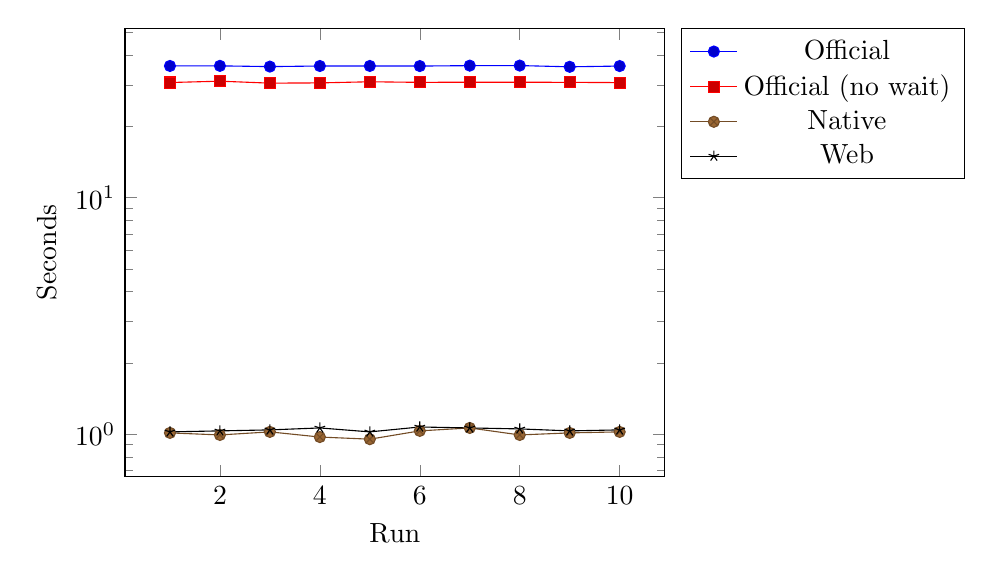
\begin{tikzpicture}
    \begin{axis}[
      ymode=log,
      ylabel=Seconds,
      xlabel=Run,
      legend pos=outer north east,
      ]
      \addplot coordinates {
        (1,  36.16)
        (2,  36.19)
        (3,  35.93)
        (4,  36.14)
        (5,  36.16)
        (6,  36.12)
        (7,  36.27)
        (8,  36.29)
        (9,  35.86)
        (10, 36.12)
      };
      \addplot coordinates {
        (1,  30.76)
        (2,  31.17)
        (3,  30.58)
        (4,  30.65)
        (5,  30.99)
        (6,  30.81)
        (7,  30.86)
        (8,  30.86)
        (9,  30.81)
        (10, 30.74)
      };
      \addplot coordinates {
        (1,  1.01)
        (2,  0.99)
        (3,  1.02)
        (4,  0.97)
        (5,  0.95)
        (6,  1.03)
        (7,  1.06)
        (8,  0.99)
        (9,  1.01)
        (10, 1.02)
      };
      \addplot coordinates {
        (1,  1.02)
        (2,  1.03)
        (3,  1.04)
        (4,  1.06)
        (5,  1.02)
        (6,  1.07)
        (7,  1.06)
        (8,  1.05)
        (9,  1.03)
        (10, 1.04)
      };
      \addlegendentry{Official}
      \addlegendentry{Official (no wait)}
      \addlegendentry{Native}
      \addlegendentry{Web}
    \end{axis}
  \end{tikzpicture}
  \caption{GASchunky benchmark (lower is faster).}%
  \label{fig:gachunky-plot}
\end{figure}

It is clearly visible that the new Emulator is several times faster than the official implementation.
On average, the official emulator without modifications takes around 36 seconds to render the full animation once.
Meanwhile the Web version of the new emulator manages to achieve the same result in just one second on average.
The native version of the new emulator which uses SDL to render the internal display is even slightly faster.
While the official emulator can be sped up drastically, it still does not come close.
This shows us that even though the new emulator only uses a single thread and runs in a browser, it still offers massive performance benefits over the official implementation.

\section{Conclusions}
\subsection{Summary}
summary with emphasis on results/comparisons
\subsection{Future work}
hardware simulator
more debugging tools
tst scripts in web ui

